\section{Result}

Assumptions were needed to be verified from the data: whether $\omega$ of all three waves agree, and the relation between $H$ and $S_{0}$ holds.

% \begin{figure}[H]
%     \centering
%     \includegraphics[width=0.48\textwidth]{images/Experiment(wthm-omega_msr)_Plate.jpg}
%     \includegraphics[width=0.48\textwidth]{images/Experiment(wthm-omega_msr)_Wave.jpg}
%     \caption{$\omega_{msr} - \omega_{thm}$ Graph of Plate(left) and Wave(right)}
%     \label{omega - omega graph1}
% \end{figure}

%https://tex.stackexchange.com/questions/11251/trend-line-or-line-of-best-fit-in-pgfplots
\begin{figure}[htbp]
    \centering
    \begin{tabular}{ll}
        \begin{filecontents*}{wthm-wwave.dat}
            wthm    wwave
            12  12.03
            12	11.91
            12	11.88
            12	11.96
            12	12.07
            12	12
            12	11.8
            12	12
            12	11.9
            12	11.77
            10	10.2
            10	10.1
            10	10.01
            10	10.07
            10	10.1
            10	10.07
            10	10.09
            10	10.05
            10	10.15
            10	9.84
            9	8.95
            9	9.02
            9	9
            9	9.02
            9	9.15
            9	9.28
            9	9.17
            9	8.94
            9	8.94
            9	8.94
            7	7.16
            7	6.99
            7	6.86
            7	6.99
            7	6.89
            7	6.85
            7	7.06
            7	6.89
            7	6.91
            7	6.9
            6	5.93
            6	5.96
            6	5.97
            6	5.94
            6	6.03
            6	5.73
            6	5.77
            6	5.76
            6	5.94
            6	5.79
            4	3.908
            4	3.984
            4	3.969
            4	3.982
            4	3.978
            4	4.082
            4	4.025
            4	4.051
            4	3.86
            4	3.784            
        \end{filecontents*}
    
        \begin{tikzpicture}[
                %Environment Cfg.
                %font=\bfseries\sffamily,
            ]
            \begin{axis}[
                width=7.5cm,
                height=7.5cm,
                at={(0,0)},
                ymin=0,
                ymax=15,
                xmin=0,
                xmax=15,
                grid=both,
                minor tick num =5,
                minor tick style={draw=none},
                minor grid style={thin,color=black!10},
                major grid style={thin,color=black!10},
                %ylabel style={rotate=90},
                ylabel={$\omega_{msr}~\left[\mathrm{rad}/s\right]$},
                xlabel={$\omega_{thm}~\left[\mathrm{rad}/s\right]$},
                tick align=outside,
                axis x line*=middle,
                axis y line*=none,
                xtick={0,2,...,16},
                ytick={0,2,...,16},
                %xlabel style={color=blue!50!cyan},
                %ylabel style={align=center,rotate=-90,color=blue!50!cyan},
                x tick label style={
                    /pgf/number format/assume math mode, font=\sf\scriptsize},
                y tick label style={
                    /pgf/number format/assume math mode, font=\sf\scriptsize},
                legend cell align = {left},
                legend pos = north west,
                legend style={nodes={scale=0.5, transform shape}},
                ]
                \addplot [only marks, 
                    mark size=1pt,
                    mark=o, 
                    %mark options={solid}, 
                    %smooth,
                    ] 
                    table [x=wthm, y=wwave] {wthm-wwave.dat};
                \addlegendentry{$ \omega_{msr}(wave) - \omega_{thm}$}
                \addplot [thick, red] table [y={create col/linear regression={y=wwave}}] {wthm-wwave.dat};
                \addlegendentry{
                    Linear regression: $ \omega_{msr} =
                    \pgfmathprintnumber{\pgfplotstableregressiona}
                    \cdot \omega_{thm}
                    \pgfmathprintnumber[print sign]{\pgfplotstableregressionb}$
                    };

                % \addplot[color=blue!50!cyan,smooth,tension=0.7,very thick] table [x index=0,y index=1,col sep=space] {Aplate-wmsrS.dat};
                % \addplot[color=cyan!50!lime,very thick] coordinates{(0,5)(25,5)};
                % \addplot[color=orange,very thick] coordinates{(0,11)(25,11)};
                % \addplot[color=red!80!orange,very thick] coordinates{(19,24.2)(23,24.2)};
                % \node[text=cyan!50!lime,fill=white,align=center,anchor=west,scale=0.8,inner sep=5pt] at (24.5,5){Base\\ Load};
                % \node[color=orange,fill=white,align=center,anchor=west,scale=0.8,inner sep=5pt] at (24.5,11){Average\\ Load};
                % \node[color=red!80!orange,fill=white,align=center,anchor=west,scale=0.8,inner sep=5pt] at (21.2,24.2){Maxium\\ Load};
            \end{axis}
        \end{tikzpicture}
        
        &
        
        \begin{filecontents}{wthm-wplate.dat}
                    wthm   wPlate
                    12	12.00
                    12	12.04
                    12	12.06
                    12	12.01
                    12	11.81
                    12	12.06
                    12	11.88
                    12	11.98
                    12	11.89
                    12	11.95
                    10	10.00
                    10	10.06
                    10	10.04
                    10	10.05
                    10	9.99
                    10	10.14
                    10	9.99
                    10	10.00
                    10	10.10
                    10	9.99
                    9	9.00
                    9	9.00
                    9	8.98
                    9	8.99
                    9	8.93
                    9	8.95
                    9	8.91
                    9	9.00
                    9	8.99
                    9	9.00
                    7	7.00
                    7	7.00
                    7	7.00
                    7	7.00
                    7	7.00
                    7	6.99
                    7	7.00
                    7	6.99
                    7	7.00
                    7	6.98
                    6	6.00
                    6	6.00
                    6	5.99
                    6	6.01
                    6	5.94
                    6	5.99
                    6	6.00
                    6	6.00
                    6	6.04
                    6	6.05
                    4	4
                    4	4
                    4	4.001
                    4	4.001
                    4	4.001
                    4	4.001
                    4	4
                    4	4
                    4	4.001
                    4	4.001   
            \end{filecontents}
        
            \begin{tikzpicture}[
                    %Environment Cfg.
                    font=\bfseries\sffamily,
                ]
                    \begin{axis}[
                        width=7.5cm,
                        height=7.5cm,
                        at={(0,0)},
                        ymin=0,
                        ymax=15,
                        xmin=0,
                        xmax=15,
                        grid=both,
                        minor tick num =5,
                        minor tick style={draw=none},
                        minor grid style={thin,color=black!10},
                        major grid style={thin,color=black!10},
                        %ylabel style={rotate=90},
                        ylabel={$\omega_{msr}~\left[\mathrm{rad}/s\right]$},
                        xlabel={$\omega_{thm}~\left[\mathrm{rad}/s\right]$},
                        tick align=outside,
                        axis x line*=middle,
                        axis y line*=none,
                        xtick={0,2,...,16},
                        ytick={0,2,...,16},
                        %xlabel style={color=blue!50!cyan},
                        %ylabel style={align=center,rotate=-90,color=blue!50!cyan},
                        x tick label style={
                            /pgf/number format/assume math mode, font=\sf\scriptsize},
                        y tick label style={
                        /pgf/number format/assume math mode, font=\sf\scriptsize},
                        legend cell align = {left},
                        legend pos = north west,
                        legend style={nodes={scale=0.5, transform shape}},
                        ]
                        \addplot [only marks, 
                            mark size=1pt,
                            mark=o, 
                            ]
                            table [x=wthm, y=wPlate] {wthm-wplate.dat};
                        \addplot [thick, red] table [y={create col/linear regression={y=wPlate}}] {wthm-wplate.dat};
                        \addlegendentry{$ \omega_{msr}(plate) - \omega_{thm}$}
                        \addlegendentry{
                            Linear regression: $ \omega_{msr} =
                            \pgfmathprintnumber{\pgfplotstableregressiona}
                            \cdot \omega_{thm}
                            \pgfmathprintnumber[print sign]{\pgfplotstableregressionb}$
                        };

                        % \addplot[color=blue!50!cyan,smooth,tension=0.7,very thick] table [x index=0,y index=1,col sep=space] {Aplate-wmsrS.dat};
                        % \addplot[color=cyan!50!lime,very thick] coordinates{(0,5)(25,5)};
                        % \addplot[color=orange,very thick] coordinates{(0,11)(25,11)};
                        % \addplot[color=red!80!orange,very thick] coordinates{(19,24.2)(23,24.2)};
                        % \node[text=cyan!50!lime,fill=white,align=center,anchor=west,scale=0.8,inner sep=5pt] at (24.5,5){Base\\ Load};
                        % \node[color=orange,fill=white,align=center,anchor=west,scale=0.8,inner sep=5pt] at (24.5,11){Average\\ Load};
                        % \node[color=red!80!orange,fill=white,align=center,anchor=west,scale=0.8,inner sep=5pt] at (21.2,24.2){Maxium\\ Load};
                    \end{axis}

        \end{tikzpicture}

    \end{tabular}
    
    \begin{tikzpicture} [remember picture, overlay]
        \node at (-5.8, 0.6) {\scriptsize{(a)}};
        \node at (2.0, 0.6) {\scriptsize{(b)}};
    \end{tikzpicture}
    \caption{$\omega_{msr} - \omega_{thm}$ graph - (a) wave (b) plate}
    \label{Experiment: omega - omega graph}
\end{figure}

Just as the assumption, $\omega$ was shared by the three waves. Both graphs of Figure \ref{Experiment: omega - omega graph} had a best-fit line with a high correlation coefficient $(R^2>0.99)$ and a slope close to 1.000. The statement 'slope = 1.0000' could be refuted by using a statistical test with $\sigma_{m}$ of the slope, but the uncertainty of the graph is relatively negligible due to the shape of the wave. It could be observed from the graphs such as Figure \ref{Data_omega=3_plate} (c). Though the wave height oscillates, it's not a clear sinusoidal wave and FFT was used to derive the dominant oscillation frequency and its amplitude. Most of the waves needed FFT analysis. The specific waveform of both waves in the channel and plate movement is provided in Appendix B, C. Also, the wave height data had intrinsic errors occurring from video tracking (Figure \ref{Tracker}).

\begin{figure}[H]
    \centering
    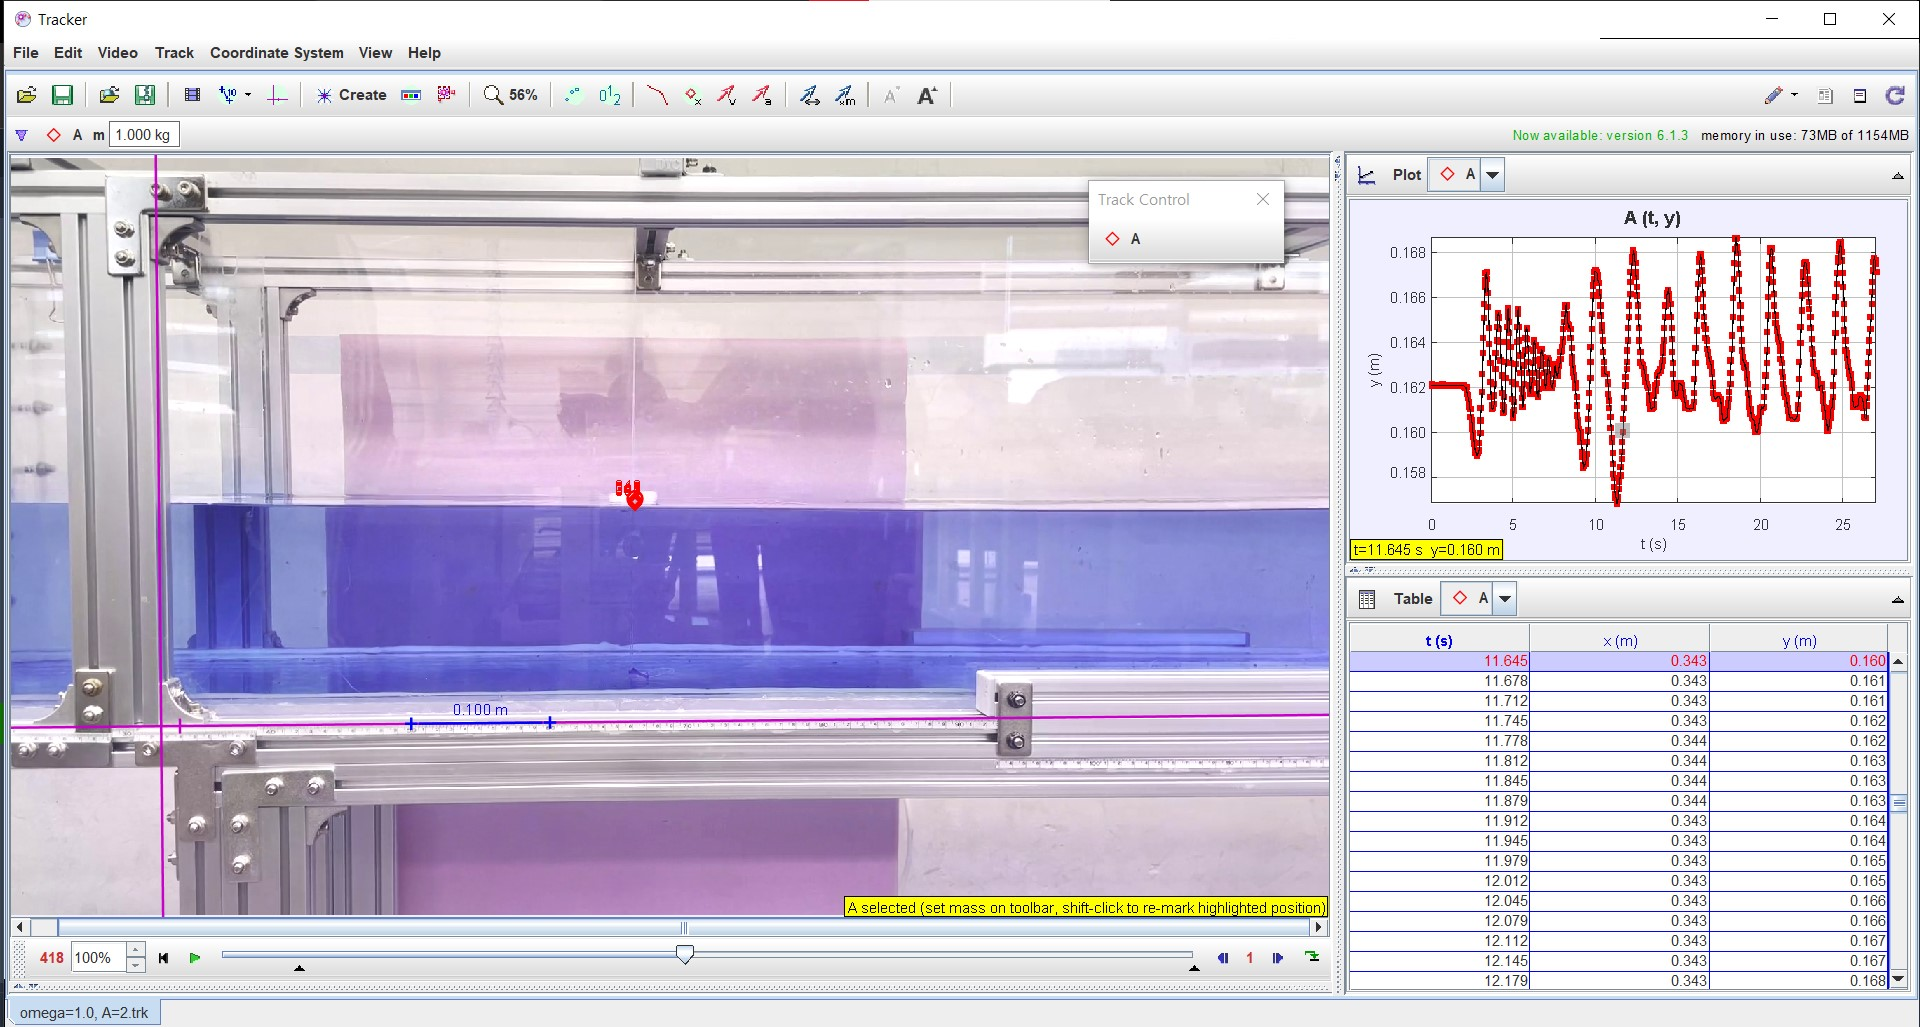
\includegraphics[width=\textwidth]{images/Experiment(Wave_Tracker, omega=1.0, A=2).jpg}
    \caption{Video Analysis}
    \label{Tracker}
\end{figure}

A black dot at one side of the buoy was tracked, but the piece of the styrofoam rotated as the wave progressed. Furthermore, the buoy submerged right under the surface on some occasions. Pointing out the surface was difficult for the cases. Testing out the data based on uncertainty is meaningless, and the statement 'slope = 1.0000' was said to be held for $\omega_{thm}$ and $\omega_{msr}$ for both plate and wave. Also, the plate moved too slowly with $\omega=3~(\sim \pi)$ that a wave was barely generated (Figure \ref{Data_omega=3_plate} (c)). The fluctuations at the front of the graph occurred from aligning the plate to the middle, and oscillation was tracked afterward: the amplitude($\sim \mathrm{cm}$) is negligible compared to the noise of the motor's rotation and its small movements.

Also, the phenomenon that $A$ decreasing as $\omega$ increasing had been observed:

\begin{figure}[H]
    \centering
        \begin{filecontents}{Aplate-wmsrS.dat}
                    wthm   A_plate
                    12	0.64
                    12	0.64
                    12	0.73
                    12	0.7
                    12	0.69
                    12	0.73
                    12	0.71
                    12	0.71
                    12	0.71
                    12	0.73
                    10	0.85
                    10	0.92
                    10	0.92
                    10	0.9
                    10	0.91
                    10	0.82
                    10	0.94
                    10	0.97
                    10	1.03
                    10	0.95
                    9	0.91
                    9	1.1
                    9	1.07
                    9	1.06
                    9	1.18
                    9	1.02
                    9	1.29
                    9	1.35
                    9	1.08
                    9	1.17
                    7	0.96
                    7	1.78
                    7	1.87
                    7	1.9
                    7	1.78
                    7	1.84
                    7	1.8
                    7	1.78
                    7	1.73
                    7	1.87
                    6	0.96
                    6	2.54
                    6	2.61
                    6	2.59
                    6	2.52
                    6	2.37
                    6	2.39
                    6	2.65
                    6	2.3
                    6	2.56
                    4	0.9566
                    4	1.913
                    4	2.856
                    4	3.795
                    4	4.744
                    4	5.313
                    4	5.568
                    4	5.662
                    4	5.677
                    4	5.681         
            \end{filecontents}
        
            \begin{tikzpicture}[
                    %Environment Cfg.
                    font=\bfseries\sffamily,
                ]
                    \begin{axis}[
                        width=0.75\textwidth,
                        height=8cm,
                        at={(0,0)},
                        ymin=0,
                        ymax=6,
                        xmin=0,
                        xmax=15,
                        grid=both,
                        minor tick num =5,
                        minor tick style={draw=none},
                        minor grid style={thin,color=black!10},
                        major grid style={thin,color=black!10},
                        %ylabel style={rotate=90},
                        ylabel={$A_{plate}~\left[\mathrm{cm}\right]$},
                        xlabel={$\omega_{msr}~\left[\mathrm{rad}/s\right]$},
                        tick align=outside,
                        axis x line*=middle,
                        axis y line*=none,
                        xtick={0,2,...,16},
                        ytick={0,1,...,6},
                        %xlabel style={color=blue!50!cyan},
                        %ylabel style={align=center,rotate=-90,color=blue!50!cyan},
                        x tick label style={
                            /pgf/number format/assume math mode, font=\sf\scriptsize},
                        y tick label style={
                        /pgf/number format/assume math mode, font=\sf\scriptsize},
                        ]
                        %\addplot[scatter, only marks] table [x index=0,y index=1,col sep=space] {Aplate-wmsrS.dat};
                        \addplot[scatter, 
                                only marks,
                                mark=o,
                                mark size=1pt,
                            ] 
                            table [x=wthm, y=A_plate] {Aplate-wmsrS.dat};
                        % \addplot[color=blue!50!cyan,smooth,tension=0.7,very thick] table [x index=0,y index=1,col sep=space] {Aplate-wmsrS.dat};
                        % \addplot[color=cyan!50!lime,very thick] coordinates{(0,5)(25,5)};
                        % \addplot[color=orange,very thick] coordinates{(0,11)(25,11)};
                        % \addplot[color=red!80!orange,very thick] coordinates{(19,24.2)(23,24.2)};
                        % \node[text=cyan!50!lime,fill=white,align=center,anchor=west,scale=0.8,inner sep=5pt] at (24.5,5){Base\\ Load};
                        % \node[color=orange,fill=white,align=center,anchor=west,scale=0.8,inner sep=5pt] at (24.5,11){Average\\ Load};
                        % \node[color=red!80!orange,fill=white,align=center,anchor=west,scale=0.8,inner sep=5pt] at (21.2,24.2){Maxium\\ Load};
                    \end{axis}
    
        \end{tikzpicture}
    \caption{$A_{plate} - \omega_{msr}$ graph}
    \label{A-omega graph}
\end{figure}

It's clear that $A_{plate}$ and $\omega_{msr}$ were negatively correlated, but the specific relation between them was not explicit: only the limiting value of $A_{plate}$ was known(since $A_{plate}$ converged as $A_{thm}$ increased).

As $\omega$ was set, it corresponds to unique $z(=kh)$ from dispersion relation:
\begin{equation}
    \omega^{2} = gk \tanh{kh} = \frac{g}{h} z ~\tanh{z}
    \label{dispersion_relation}
\end{equation}

The $z$ from Equation \ref{dispersion_relation} is the same value as the one in Equation \ref{eq_023}, and $H/S_{thm}$ could be derived. It was compared with $H/S_{msr}$, which could be calculated from the data set (Figure \ref{H/S graph}).

% \begin{figure}[H]
%     \centering
%     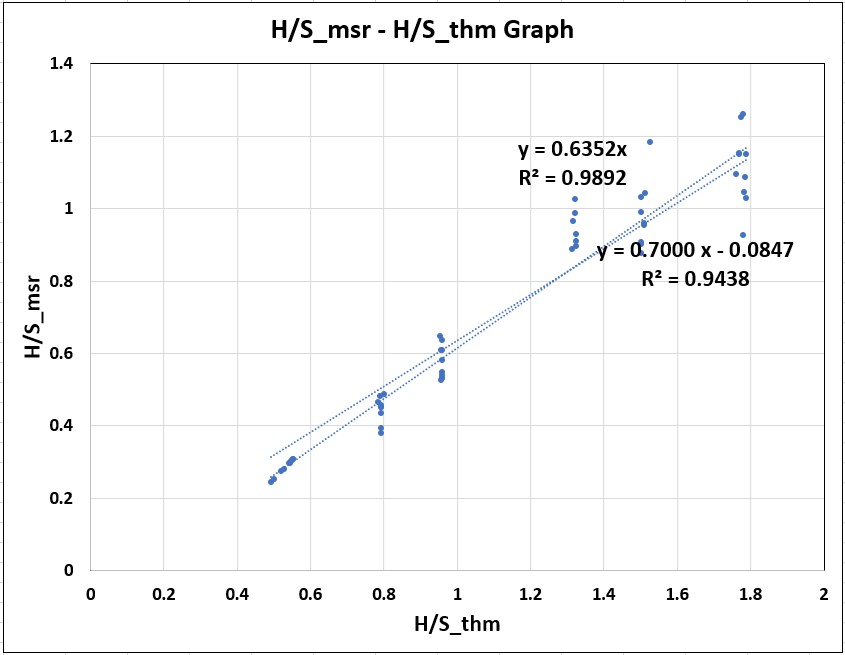
\includegraphics[width=\textwidth]{images/Experiment(H.S_thm-H.S_msr)_Proccessed_Data.jpg}https://www.overleaf.com/project/63aff5462256d537ece5848a
%     \caption{Caption}
%     \label{fig:enter-label1}
% \end{figure}

%https://tex.stackexchange.com/questions/11251/trend-line-or-line-of-best-fit-in-pgfplots
\begin{figure}[htbp]
    \centering
        \begin{filecontents}{HSthm-HSmsr.dat}
                HS_thm	HS_msr
                1.781440728	0.925436527
                1.785651376	1.085170025
                1.787735635	1.027713311
                1.782498659	1.045913291
                1.760671425	1.094309648
                1.787735635	1.15104453
                1.768471166	1.150212766
                1.77931432	1.26011236
                1.769571325	1.151819856
                1.776098332	1.252500343
                1.502818971	0.907053163
                1.512879552	1.042827713
                1.509535179	0.952282833
                1.51120852	0.957989748
                1.501134272	0.989520132
                1.526163172	1.182451424
                1.501302842	1.031007752
                1.502482211	0.900403351
                1.519540335	0.724198251
                1.501134272	0.877353529
                1.324569679	0.909190732
                1.324937643	0.929155313
                1.321072373	0.986915888
                1.323465588	1.024621212
                1.313331279	0.887096774
                1.315913161	0.964838394
                1.309086454	0.733436773
                1.326041332	0.895167286
                0.958556795	0.531089978
                0.958906454	0.580898876
                0.959081306	0.608042895
                0.958731617	0.530870712
                0.959081306	0.635545557
                0.956634768	0.607395324
                0.959431056	0.540311804
                0.95646013	0.524718468
                0.958556795	0.547893826
                0.954714602	0.645610278
                0.792888221	0.451327434
                0.792888221	0.377926685
                0.790392394	0.481381958
                0.793981875	0.44980695
                0.783557379	0.464839094
                0.791639619	0.434911243
                0.792419834	0.455155071
                0.79195164	0.393355983
                0.798366989	0.608601216
                0.800094292	0.48515625
                0.492276411	0.242943759
                0.528893957	0.280658651
                0.543862815	0.296883754
                0.553908234	0.308036891
                0.552905492	0.306913997
                0.542089448	0.294936947
                0.546948794	0.300287356
                0.551047756	0.304839279
                0.521368486	0.272679232
                0.499818992	0.25048407                  
            \end{filecontents}
        
            \begin{tikzpicture}[
                    %Environment Cfg.
                    font=\bfseries\sffamily,
                ]
                    \begin{axis}[
                        width=\textwidth,
                        height=10cm,
                        at={(0,0)},
                        ymin=0,
                        ymax=1.4,
                        xmin=0,
                        xmax=2,
                        grid=both,
                        minor tick num =5,
                        minor tick style={draw=none},
                        minor grid style={thin,color=black!10},
                        major grid style={thin,color=black!10},
                        %ylabel style={rotate=90},
                        ylabel={$H/S_{msr}$},
                        xlabel={$H/S_{thm}$},
                        tick align=outside,
                        axis x line*=middle,
                        axis y line*=none,
                        xtick={0,0.2,...,2},
                        ytick={0,0.2,...,2},
                        %xlabel style={color=blue!50!cyan},
                        %ylabel style={align=center,rotate=-90,color=blue!50!cyan},
                       x tick label style={
                            /pgf/number format/assume math mode, font=\sf\scriptsize},
                        y tick label style={
                            /pgf/number format/assume math mode, font=\sf\scriptsize},
                        legend cell align = {left},
                        legend pos = north west,
                        legend style={nodes={scale=0.5, transform shape}},
                        ]
                        \addplot[scatter, 
                                only marks, 
                                mark=o,
                                mark size=1.5pt,
                                color=black,
                            ] 
                        table [x=HS_thm, y=HS_msr] {HSthm-HSmsr.dat};    
                        \addplot [thick, red] table [y={create col/linear regression={y=HS_msr}}] {HSthm-HSmsr.dat};
                        %\addlegendentry{$y(x)$}
                        \addlegendentry{
                            Linear regression: $ \omega_{msr} =
                            \pgfmathprintnumber{\pgfplotstableregressiona}
                            \cdot \omega_{thm}
                            \pgfmathprintnumber[print sign]{\pgfplotstableregressionb}$
                        };

                        % \addplot[color=blue!50!cyan,smooth,tension=0.7,very thick] table [x index=0,y index=1,col sep=space] {Aplate-wmsrS.dat};
                        % \addplot[color=cyan!50!lime,very thick] coordinates{(0,5)(25,5)};
                        % \addplot[color=orange,very thick] coordinates{(0,11)(25,11)};
                        % \addplot[color=red!80!orange,very thick] coordinates{(19,24.2)(23,24.2)};
                        % \node[text=cyan!50!lime,fill=white,align=center,anchor=west,scale=0.8,inner sep=5pt] at (24.5,5){Base\\ Load};
                        % \node[color=orange,fill=white,align=center,anchor=west,scale=0.8,inner sep=5pt] at (24.5,11){Average\\ Load};
                        % \node[color=red!80!orange,fill=white,align=center,anchor=west,scale=0.8,inner sep=5pt] at (21.2,24.2){Maxium\\ Load};
                    \end{axis}
        \end{tikzpicture}
    \caption{$H/S_{msr} - H/S_{thm}$ graph}
    \label{H/S graph}
\end{figure}

